\documentclass[letterpaper,10pt]{article}

\usepackage{enumitem}
\usepackage{titling}
\usepackage{listings,listings-rust}
\usepackage{url}
\usepackage{soul}
\usepackage{hyperref}
\usepackage{setspace}
\usepackage{subfig}
\usepackage{sectsty}
\usepackage{pdfpages}
\usepackage{colortbl}
\usepackage{multirow}
\usepackage{multicol}
\usepackage{relsize}
\usepackage{amsmath}
\usepackage{wasysym}
\usepackage{fancyvrb}
\usepackage[yyyymmdd]{datetime}
\usepackage{amsmath,amssymb,amsthm,graphicx,xspace}
\usepackage[titlenotnumbered,noend,noline]{algorithm2e}
\usepackage[compact]{titlesec}
\usepackage{XCharter}
\usepackage[T1]{fontenc}
\usepackage[scaled]{beramono}
\usepackage[normalem]{ulem}
\usepackage{booktabs}
\usepackage{tikz}
\usetikzlibrary{arrows.meta,automata,shapes,trees,matrix,chains,scopes,positioning,calc,decorations.pathreplacing}
\tikzstyle{block} = [rectangle, draw, fill=blue!20, 
    text width=2.5em, text centered, rounded corners, minimum height=2em]
\tikzstyle{bw} = [rectangle, draw, fill=blue!20, 
    text width=4em, text centered, rounded corners, minimum height=2em]

\definecolor{namerow}{cmyk}{.40,.40,.40,.40}
\definecolor{namecol}{cmyk}{.40,.40,.40,.40}
\renewcommand{\dateseparator}{-}

\let\LaTeXtitle\title
\renewcommand{\title}[1]{\LaTeXtitle{\textsf{#1}}}

\lstset{basicstyle=\footnotesize\ttfamily,breaklines=true}

\newcommand{\CPP}{C\nolinebreak\hspace{-.05em}\raisebox{.4ex}{\tiny\bf +}\nolinebreak\hspace{-.10em}\raisebox{.4ex}{\tiny\bf +}}
\def\CPP{{C\nolinebreak[4]\hspace{-.05em}\raisebox{.4ex}{\tiny\bf ++}}}

\newcommand{\handout}[5]{
  \noindent
  \begin{center}
  \framebox{
    \vbox{
      \hbox to 5.78in { {\bf ECE459: Programming for Performance } \hfill #2 }
      \vspace{4mm}
      \hbox to 5.78in { {\Large \hfill #4  \hfill} }
      \vspace{2mm}
      \hbox to 5.78in { {\em #3 \hfill \today} }
    }
  }
  \end{center}
  \vspace*{4mm}
}

\newcommand{\lecture}[3]{\handout{#1}{#2}{#3}{Lecture#1}}
\newcommand{\tuple}[1]{\ensuremath{\left\langle #1 \right\rangle}\xspace}

\addtolength{\oddsidemargin}{-1.000in}
\addtolength{\evensidemargin}{-0.500in}
\addtolength{\textwidth}{2.0in}
\addtolength{\topmargin}{-1.000in}
\addtolength{\textheight}{1.75in}
\addtolength{\parskip}{\baselineskip}
\setlength{\parindent}{0in}
\renewcommand{\baselinestretch}{1.5}
\newcommand{\term}{Winter 2020}

\singlespace


\begin{document}

\lecture{30 --- Introduction to Queueing Theory}{\term}{Jeff Zarnett}

\section*{A Short Introduction to Queueing Theory}

Queueing theory is literally the theory of queues---what makes queues appear, how will they behave, and how do we make them go away? Queueing theory has played a role in your life whether you know it or not: this is how tech support at Rogers or Bell or Telus or whomever decides just how many customer service agents to have available at any given time. Of course, your local telecom chooses to minimize the number of employees at the cost of making you wait (``Your call is important to us; please hold while we ignore it.'') but they study carefully how much waiting is too much waiting and how much is too little. Queueing theory is applicable to lots of fields, including industrial design, call centres, telecom systems, and computers executing transactions. 

To scale up a system, we have a lot of choices to make, and these will work best if they are supported by data. Queueing theory helps us decide what's best. Here are a few possible examples, from~\cite{pmd}:

\begin{itemize}
 \item Given a choice between a single machine with speed $s$ or $n$ machines, each with speed $s/n$, which should we choose?
 \item If the arrival rate and service rate double, how does the mean response time change?
 \item Should we try to balance load or is that a waste of time/effort?
 \item Can we give priority to certain operations without harming another category of job?
 \item How do job size variability and heavy-tailed workloads affect our choices of scheduling policy?
 \item If 12 servers is enough to handle 9 jobs per second, do we need 12~000 servers if we have an arrival rate if 9~000 jobs per second?
\end{itemize}

I tend to tell stories about banks that imply I hate them. Not really, they're just a place where there's likely to be a queue and I'm likely to be annoyed and thinking about how to optimize this situation. So let's define some terms formally, to make sure we're all on the same page when it comes to terminology and language. Some of these will seem obvious, but let's be complete (like the book~\cite{swps}):

\begin{itemize}
	\item Server - The banking centre fulfilling customer requests.
	\item Customer - Initiator of service requests.
	\item Wait time - The time a customer spends waiting in line.
	\item Service time - The time from when a teller starts to serve a customer up to the time when the next customer is called forward.
	\item Arrival rate - The rate at which customers arrive.
	\item Service rate - the rate at which customer requests are serviced.
	\item Utilization - The fraction of the teller's time used actually handling customer requests (not idling).
	\item Queue length - The total number of customers waiting, or currently with a teller, or both.
	\item Response time - The sum of wait and service time for a single visit.
	\item Residence time - The total response time if a customer visits several tellers (or the same one multiple times).
	\item Throughput - The rate at which customers get their requests serviced and dealt with.
\end{itemize}

The mathematical symbols for this are represented in the following table~\cite{swps}:


\begin{center}
	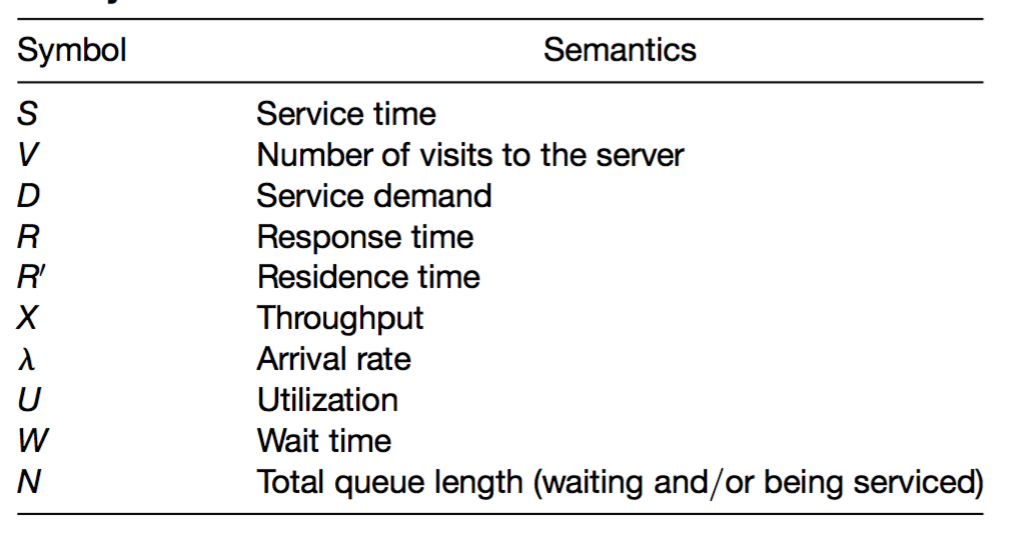
\includegraphics[width=0.65\textwidth]{images/math-symbols.png}
\end{center}

If you're cynical like me, you will think the bank works very hard to not have tellers in the bank to maximize your wait time and minimize their staffing costs. It's actually (allegedly) a trade-off: if I have to wait too long to do my banking, I could always take my business elsewhere (but is that likely to happen?). Minimizing customer wait time makes customers happy, so that's something the bank should want. It would also be nice if the bank trains its tellers well, so they can complete all operations, even unusual ones, quickly and efficiently, reducing the service time. The bank is not a charity operation so they will of course want to minimize staffing, but it knows that overstaffed is bad and understaffed is also bad. 

Back to the realm of computers: you have lots of queues in your computer. The CPU uses a time-sharing scheduler to run as many concurrent programs as possible. A router has a queue for packets (data) that has a maximum size, and if this is exceeded, packets will be simply dropped. 

Queueing theory gives us a formal framework with which to grapple with our problems instead of just guessing. Remember how bad we are at guessing. 


\paragraph{Example.} Let's look at a simple example from~\cite{pmd}. Imagine we have a system with one CPU that serves a queue of jobs in First-Come-First-Served (FCFS) order with an arrival rate $\lambda$ of 3 jobs per second. Each job takes some amount of time and resources, but we can ignore the particulars for right now. Suppose the average service rate $\mu$ is 5 jobs per second (or stated another way, the average job requires $0.2s$ to service). The system is not overloaded: 3 jobs per second arriving is less than 5 jobs per second being serviced. Our terminology for describing the mean response time will be $E[T]$. 


Suppose now that your boss says that tomorrow the arrival rate will double. If you do nothing, you can imagine, there will be a problem: we would have 6 jobs arriving per second, on average, to a system that can service, on average, 5 jobs per second. You have been allocated some budget to replace the CPU with a faster one, and you should choose one so that the jobs still have a mean response time of $E[T]$. This situation is depicted below~\cite{pmd}:


\begin{center}
	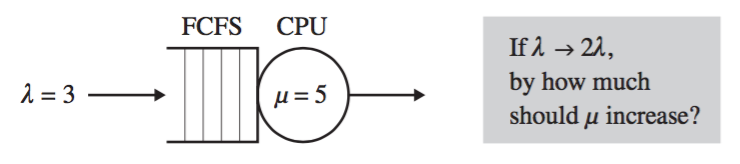
\includegraphics[width=0.5\textwidth]{images/qt-example1.png}
\end{center}

That is, customers should not notice the increase in arrival rate. So, should we (1) double the CPU speed; (2) more than double the CPU speed; or (3) less than double the CPU speed?

The answer is (3): we don't need to double the CPU speed. We can see later in formal terms why this is the case, but think for a minute about why it is? If we double the service rate and double the arrival rate, we actually get half the mean response time...

\paragraph{Example 2.} Okay, how about another example from~\cite{pmd}. There are always $N=6$ jobs running at a time. As soon as a job completes, a new one is started (this is called a \textit{closed system}). Each job goes through to be processed on one of two servers (and it is 50-50 where the job ends up), each of which has a service time $\mu$ of 1 job per 3 seconds. Again, depicted below~\cite{pmd}:


\begin{center}
	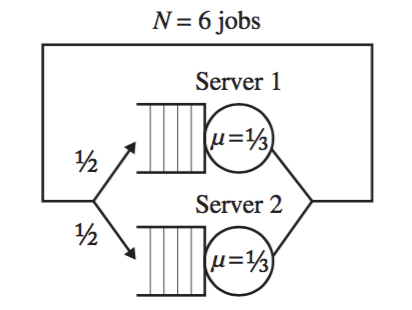
\includegraphics[width=0.3\textwidth]{images/qt-example2.png}
\end{center}

Bad news: sometimes, improvements do nothing. If we replace server one which is twice as fast (so 2 jobs per 3 seconds), does that help? Nope. Not really. Does raising $N$ help? Nope, negligible effect. The bottleneck device is the limiting factor. Strangely, dropping $N$ to 1 means the server replacement makes a difference, if you can call that improvement. 

What if it's an \textit{open system} where arrival times are independent of completion, as below~\cite{pmd}?


\begin{center}
	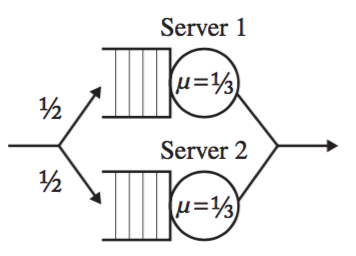
\includegraphics[width=0.3\textwidth]{images/qt-example2-2.png}
\end{center}

In this case, yes, replacing server 1 makes a huge difference!

\paragraph{Example 3.} A third example, this time addressing directly the question of do we want one fast server or $n$ slower ones? Horse-sized duck and duck-sized horses jokes aside, what is better if we want to minimize the mean response time when we have non-preemptable jobs (i.e., once started, a job has to run to completion and cannot be interrupted)~\cite{pmd}:


\begin{center}
	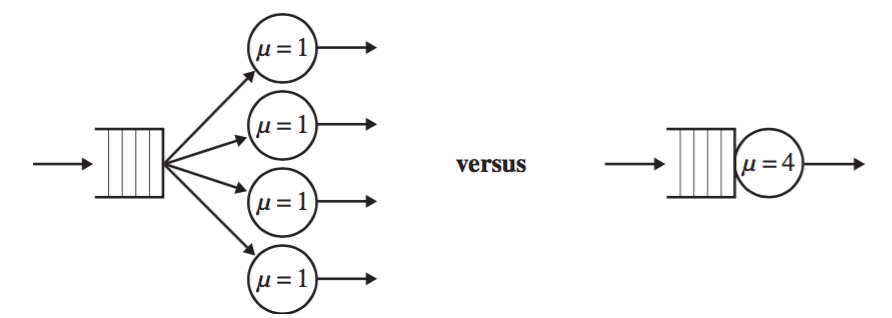
\includegraphics[width=0.6\textwidth]{images/qt-example3.png}
\end{center}

The answer is ``it depends''. That's frustrating, but this is Sparta. Or at least, real life. One big factor is the variability of the job sizes. Imagine you are at the grocery store and most people have 12 items or fewer\footnote{Not less. Fewer. It is countable; therefore fewer. Yes, I am obsessive about this.} and there's one guy who's buying 85 items. You don't want to be standing in line with milk and eggs behind someone who is trying to buy six of everything, do you? So if there's high variability, you probably want multiple servers -- the guy buying the whole store can hold up line \#1 and you can go to line \#4 and you're out and done before he is finished.

What if the load is low? Chances are you would prefer the one fast server instead of having some number of servers doing nothing.

What if jobs are interruptible (preemptible)? You could always use a single fast machine to simulate $n$ slow machines, so a single fast machine is at least as good as the alternative. 

\subsection*{A Digression on Load Balancing}

Imagine your typical ``server farm'' - you have $n$ servers that are all responsible for handling incoming requests. Let's imagine all servers are the same (or close enough). What we typically see in load balancing is assignment of tasks to servers via some dispatcher~\cite{pmd}:

\begin{center}
	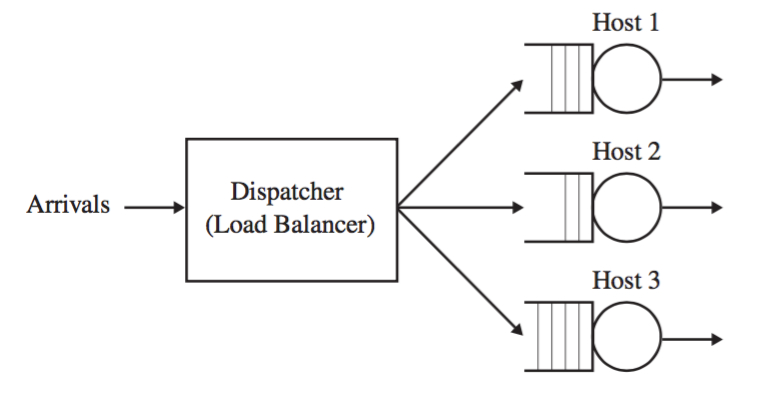
\includegraphics[width=0.6\textwidth]{images/central-dispatcher.png}
\end{center}

This isn't the only kind of load balancing we can do; there is also the ability to do after-the-fact assignment (or work-stealing), which consists of monitoring the various queues and reassigning work if it's piling up somewhere.

There are a few different task assignment policies---ways in which we can assign work to servers~\cite{pmd}:

\begin{itemize}
	\item Random: Exactly what it sounds like.
	\item Round-Robin: The $i$th job goes to host $i$ modulo $n$.
	\item Shortest-Queue: The job goes to the server with the shortest queue.
	\item Size-Interval-Task-Assignment: Short jobs go to one server, medium to another, long to another...
	\item Least-Work-Left: A job goes to the server that has the least total remaining work, where work is the sum of the size of the jobs.
	\item Central-Queue: Rather than being assigned to a host directly, when a server needs work to do, it gets the first job in the central queue.
\end{itemize}

Which of these policies yields the lowest mean response time? Answer: truthfully, nobody knows. It depends, of course, on your job variability and and that sort of thing, but it hasn't been well studied. PhD, anyone?

\subsection*{Red Line Overload\footnote{You've seen ``Top Gun'', right? \url{https://www.youtube.com/watch?v=siwpn14IE7E}}}

Earlier I mentioned it would probably be bad to see 6 jobs arriving per second to a system that can handle 5 per second. This doesn't seem like rocket science, but it bears repeating. In our discussion we require that $\lambda \leq \mu$ and assume that $\lambda < \mu$. That is to say, we are not overloaded (as engineering students you may be amused by the idea that you might one day NOT be overloaded). Remember now that the values for $\lambda$ and $\mu$ are averages, so it could happen that temporarily we ``fall behind'' a bit, but then make up for it a little later on, or we temporarily get ahead before a bunch more work gets piled on. Think about the long term, though -- if we are not at least keeping up then this will eventually get out of hand. How badly? Well, in the limit, the queue length goes to infinity.

The justification comes from~\cite{pmd}: Let's represent time with $t$, its usual symbol and define $N(t)$ as the number of jobs in the system at time $t$. $A(t)$ represents arrivals by time $t$ and $D(t)$ represents departures by time $t$. So:

\begin{center}
	$E[N(t)] = E[A(t)] - E[D(t)] \geq \lambda t - \mu t = t (\lambda - \mu) $
\end{center}

The tiniest bit of calculus says that if arrivals exceed departures, taking the limit as $t$ goes to infinity means $t (\lambda - \mu) $ also goes to infinity. Whoops. So to prevent this terrible situation we just happily assume that this doesn't happen\footnote{I'm reminded of a funny engineering saying that says if you encounter a system that is nonlinear, you can decide that nonlinear systems are too difficult to reason about, assume the system is linear, and proceed.}. 

Raising $\mu$ is generally desirable. This is, after all, programming for performance -- the faster we complete work, the more work we can get done in the same amount of time. Improving the service rate, however, does not necessarily improve the throughput. 

Wait, what? We've assumed that the arrival rate is less than the service rate. So we have enough capacity to handle all incoming work. So the limiting factor on completed work is actually arriving work. We have the capacity to do at least what is arriving and possibly a bit more. Adding more work capacity doesn't mean more work gets done if there isn't any more work to do. You might be capable of completing six assignments for this class in a term, but if you're (mercifully) only assigned four, then you will only complete four. So raising $\mu$ increases the maximum possible throughput, but does not necessarily increase the actual throughput.

But just to make you suffer, things are very different in a closed system: one in which there is always more work to do and as soon as one item is finished the next one enters the queue. This is the case in batch systems. You know, the old mainframe kind of processing where you submit your job to be run overnight and in the morning you get a result. Hopefully the one you wanted. In that case, we are running at capacity all the time, so actually $\mu$ is the controlling factor -- the throughput is exactly the service rate. 

Not that open networks are particularly intuitive, but closed networks can kind of mess with our intuition in general. Imagine we have a closed system with Multiprogramming Level (MPL) of $N$ as below~\cite{pmd}:

\begin{center}
	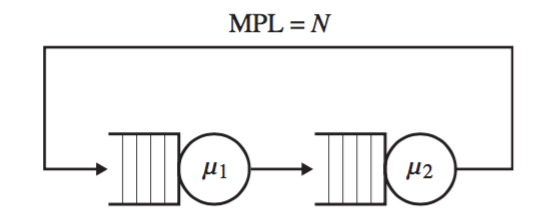
\includegraphics[width=0.4\textwidth]{images/tandem-closed.png}
\end{center}

What is the throughput here? Intuition suggests min($\mu_{1}, \mu_{2}$), right? Sometimes. This is okay if the slower server is always busy, but that's not always the case. What if $N$ is 1? Okay, that's a bit of an exception case though. What about $N$ being 2? Then the slower server has some work to do at all times right? Nope, sadly not. Sometimes the slow server is faster than the fast server, because $\mu_{1}$ and $\mu_{2}$ are just averages. And averages can be misleading! The average family might have 2.3 children (or whatever the figure is), but you can't exactly have 0.3 of a child...

\subsection*{Don't Guess...}
One final anecdote from~\cite{pmd} on the subject of measuring $\mu$. Some smart folks at IBM wanted to know, given the arrival rate $\lambda$, what the mean job size, $E[S]$ (which is $1/\mu$) was. Well, $E[S]$ is the mean time required for a job in isolation, so our experiment should be a hundred runs of sending a single job into the system and averaging the values. This is okay, but does not reflect reality where we have things like caching of data and multiple concurrent jobs. There are two basic strategies we can follow, depending on whether it is an open or closed system for getting a value for $\mu$, allowing simple computation of $E[S]$.

The open system strategy is: ramp up $\lambda$. Keep piling more jobs on the system. At some point the system will not be able to keep up. Once the completion rate levels off, we hit the limit and we have a value for $\mu$.

The closed system strategy: set it up so there is always work to do. In closed systems, there's often consideration given to \textit{think time} -- this is what happens when the user is on the command line and dispatching work to do. The user sends a command and awaits a result. After the result, some time passes while the user decides what to do next (or does code editing before running the compiler again). To keep the system totally busy in the stress test, we need think time to be zero -- so additional work is always available. And then we can simply measure the jobs completing per second, giving us $\mu$ directly.

\bibliographystyle{alphaurl}
\bibliography{459}


\end{document}
practical queueing theory:  https://www.youtube.com/watch?v=IPxBKxU8GIQ
